\cleardoublepage
\chapter{Introduksjon}
\label{chap:intro}

\section{Bakgrunn for prosjektet}
Det kommer frem i Studentenes Helse -og Trivselsundersøkelse (SHoT-undersøkelsen) fra 2018 at nesten hver tredje student opplever ensomhet i studietiden. I tillegg rapporterer hver fjerde student at de opplever alvorlige psykiske plager, sammenlignet med SHoT-undersøkelsen fra 2010, da dette kun gjaldt hver sjette student \cite{SHOT:2}. For å styrke psykisk helse og livskvalitet råder Helsedirektoratet blant annet til å knytte bånd med andre gjennom å delta som frivillig i lokale initiativ og organisasjoner\footnote{\url{https://helsenorge.no/psykisk-helse/fem-rad-for-sterkere-psykisk-helse}} og nevner satsning på sosial aktivitet og deltakelse som viktig for folkehelsen\footnote{\url{https://www.helsedirektoratet.no/faglige-rad/lokale-folkehelsetiltak-veiviser-for-kommunen/psykisk-helse-og-livskvalitet-lokalt-folkehelsearbeid/tiltak-og-virkemidler/stimulere-til-aktivitet-og-deltakelse}}. 

Å legge til rette for studenters deltakelse i lokale lag, foreninger og organisasjoner vil støtte opp under Helsedirektoratets satsningsområder innenfor folkehelse. Tilhørighet til stedet man bor er også viktig, spesielt for tilflyttende studenter. Tiltak rettet mot tilflyttere til kommunene for å holde på disse er sentralt for utvikling og verdiskaping i lokalsamfunnet\footnote{\url{https://www.regjeringen.no/no/tema/kommuner-og-regioner/regional--og-distriktspolitikk/lokal-samfunnsutvikling1/id2350748/}}. Å oppfordre til at studenter deltar i nærmiljøet og knytter bånd med lokalbefolkningen over felles interesser er et tiltak rettet mot både tilflyttere og studiekommunenes lokalbefolkning. Av disse grunnene vil det være ønskelig å utforme en løsning for et lavterskel-tilbud der studenter ved Høgskolen i Østfold (omtalt som {\em HIØ} videre i dokumentet) skal kunne finne, kontakte og delta i lokale lag, foreninger og organisasjoner.

Gjennom bruk av metodikk knyttet til fagområdene Informasjonsarkitektur og Brukerorientert Design skal det utformes en digital løsning kalt {\em Aktiv Student} som kan benyttes av studenter ved HIØ for å få oversikt over fritidstilbudet innen lokale lag, foreninger og organisasjoner (også omtalt kun som {\em organisasjoner} videre i dokumentet). Prosjektets samfunnsmessige bakgrunn og menneskelige aspekt skal benyttes som retningslinjer under utformingen av løsningen med formål om å skape et lavterskel-tilbud som studenter ved HIØ ønsker å benytte seg av.

\subsection{Problemstilling}
Studenter ved HIØ har pr. i dag ikke tilfredsstillende verktøy for å finne oversikt over fritidsaktiviteter og ta kontakt med organisasjoner som arrangerer disse. Hvordan kan man designe et verktøy som legger til rette for at studenter enklere kan delta på fritidsaktiviteter og ta kontakt med organisasjoner, lag og foreninger i sitt nærområde? Hvordan kan tjenesten utformes på en måte som gjør det interessant og attraktivt for studenter å gjøre dette? Hvordan kan denne tjenesten synliggjøres for både studenter og organisasjoner, lag og foreninger med den hensikt at den skal bli brukt av majoriteten av målgruppen?

\section{Prosjektgruppen}
Denne oppgave er utarbeidet og gjennomført av fire studenter ved avdeling for informasjonsteknologi ved Høgskolen i Østfold.

\begin{center}
\begin{tabular}{ l l }
 Ingrid Elise Dahl & Studerer: Informatikk \\ 
 Markus Arnø Madsen & Studerer: Digitale medier og Design \\  
 Anders Walle Pettersen & Studerer: Digitale medier og Design \\
 Stefan Larsen & Studerer: Digitale medier og Design \\
\end{tabular}
\end{center}

\section{Oppdragsgiver}
Prosjektgruppens oppdragsgiver er Tommy Payne på vegne av HIØ. Tommy Payne jobber som Seniorkonsulent i Studieenheten ved HIØ og medvirker i team for Studieutredning og kvalitetssikring med ansvar for det helhetlige læringsmiljøet ved campus Halden og campus Fredrikstad. Arbeidet hans går ut på å sikre og videreutvikle det digitale, fysiske, organisatoriske og psykososiale læringsmiljøet ved HIØ. \footnote{https://www.hiof.no/om/organisasjon/administrasjonen/organisasjons-og-tjenesteutvikling/studenttjenester/personer/tekn-adm-ansatte/tommypa/}

\section{Oppdraget}
Løsningen som gruppen og oppdragsgiver kom frem til er å utvikle en prototype av en nettbasert tjeneste for studenter der de kan finne organisasjoner, lag og foreninger i sitt nærområde. Prototypen skal bestå av et sett med interaktive skisser laget i verktøyet Adobe XD. Prosjektet baserer seg på at gruppen skal levere denne prototypen sammen med hoveddokumentet til oppdragsgiver, hvor disse kan fungere som et utgangspunkt for å muliggjøre utviklingen av prototypen til en fullverdig tjeneste på et senere tidspunkt. En av funksjonene som skal inkluderes i prototypen er innhenting av informasjon om organisasjoner, lag og foreninger fra Brønnøysundregistrene \footnote{https://www.brreg.no/}, i tillegg til en løsning som oppfordrer organisasjoner til å føre opp utfyllende informasjon om seg selv.

Løsningen skal også ivareta de sosiale og menneskelige aspektene ved å oppfordre til kommunikasjon mellom studenter og kontaktpersoner for organisasjoner, på en enkel og ikke-truende måte. Løsningen skal tilrettelegge for at det skal være enkelt å delta på aktiviteter sammen med andre studenter. I tillegg skal løsningen kunne foreslå potensielt interessante organisasjoner til studenter som ønsker dette.

Oppdragsgiver Tommy Payne jobber med læringsmiljø og studentenes trivsel og helse ved HIØ. Oppdragsgivers fokus på inkludering og trivsel fører denne oppgaven mot å utvikle en løsning som kan bidra til at studenter blir mer aktive, deltar mer sosialt og engasjerer seg i lokalmiljøet. Dette er av interesse for både studentene, Tommy Payne, HIØ og nærmiljøet rundt skolen.

\subsection{Formål}
\label{sec:maal-metode-resultater}

\begin{compactitem}
\item [{\bf Hovedmål}] Målet med prosjektet er å designe en løsning for at studenter ved HIØ enklere kan få oversikt over og komme i kontakt med frivillige organisasjoner, lag og foreninger i sitt nærområde, samt designe en bedre og enklere løsning enn den som finnes idag.
\begin{compactitem}
\item [{\bf  Delmål 1: Studentaspektet} ] Designe en løsning med den hensikt å gjøre det enklere for studenter ved HIØ å finne og å komme i kontakt med organisasjoner, lag og foreninger i nærområdet, samt andre studenter med like interesser. Tilby lavterskel muligheter for sosialisering og fellesskap for alle studenter ved HIØ som på lang sikt kan virke positivt inn på studentengasjementet.
\item [{\bf  Delmål 2: Organisasjonsaspektet} ] Designe en løsning med den hensikt å gjøre det enklere for lokale organisasjoner, lag og foreninger å bli sett av studenter ved HIØ for å tilrettelegge for økt medlemstall og større engasjement i organisasjonene.
\item [{\bf  Delmål 3: Samfunnsaspektet} ] Designe en løsning som legger opp til å kunne skape kontaktpunkter mellom studenter og fastboende i studiekommunene, som på lang sikt kan bidra til å skape tilhørighet for studenter, øke engasjementet og motivasjonen til å bidra i sitt nærområde.
\item [{\bf  Delmål 4: Synlighetsaspektet} ] Utforme en plan for å skape en tjeneste som alle studenter ved HIØ og organisasjoner i nærområdet vet eksisterer og vet hvor de kan finne. Designe en løsning som studenter og organisasjoner selv ønsker å bruke og ser verdien og nytten ved.
\end{compactitem} 
\end{compactitem}

\subsection{Utvikling av hypoteser}
\label{section:hypoteser}
Prosjektgruppen utviklet fire hypoteser som i løpet av prosjektet ble utforsket gjennom brukerintervjuer -og undersøkelser, forskning og samtaler med fagpersoner. I utviklingen av hypotesene la prosjektgruppen vekt på det sosiale og samfunnsmessige aspektet i tillegg til det tekniske aspektet. Grunnlaget for dette var at det sosiale og samfunnsmessige aspektet med tjenesten var et viktig fokusområde for oppdragsgiver. Derfor burde prosjektgruppens funn innen dette området ligge til grunn for tekniske og designrelaterte beslutninger tatt under utformingen av tjenesten.

Hypotesene fungerte som ledetråder for prosjektgruppen i arbeidet med å utforme prototypen. I brukerundersøkelsene ble spørsmål og tematikk vinklet mot innholdet i hypotesene ettersom hypotesene oppsummerte prosjektgruppens tanker og antakelser om hva som var viktigst å legge vekt på i tjenesten. Om noen av disse antakelsene i løpet av undersøkelsene ble motbevist eller fikk liten støtte ville det føre til at temaene i brukerundersøkelsene måtte vinkles annerledes.

\paragraph{Hypoteser}
\begin{compactitem}
\item[{\bf H1}] En tjeneste som tilrettelegger for å delta sammen med andre likesinnede kan senke terskelen for å delta på en aktivitet.
\item[{\bf H2}] Studenter ved HIØ synes det er vanskelig å finne en oversikt over aktivitetstilbud
\item[{\bf H3}] Studenter ved HIØ synes terskelen for å selv ta kontakt med organisasjoner og aktivitetsgrupper er for høy 
\item[{\bf H4}] Spennende funksjoner og godt design skaper en tjeneste som studenter ved HIØ ønsker å benytte
\end{compactitem}



\section{Analyse}
Det ble gjennomført en analyse av relatert arbeid og relevante tjenester. Disse blir i dette delkapittelet evaluert og sammenlignet opp mot prosjektoppgaven. Hensikten med dette var å finne ut av hva som allerede eksisterte i markedet. Hvordan det fungerer, hva som ikke fungerer og hvordan prosjektgruppens løsning kan skille seg ut fra det som eksisterer. 

\subsection{Målgruppen}
I prosjektbeskrivelsen gitt av oppdragsgiver, vedlagt i Tillegg~\ref{vedlegg:prosjektbeskrivelse} beskrives den tiltenkte målgruppen for den ferdig utviklede tjenesten Aktiv Student. Målgruppen for tjenesten er satt til å være studenter ved HIØ, som vil kunne bruke tjenesten for å få en oversikt over lokale organisasjoner, lag og foreninger og kunne komme i kontakt med disse. Utover dette skal løsningen også kunne brukes av lokale organisasjoner, lag og foreninger. Disse vil kunne bruke tjenesten til å øke sin synlighet og som en kommunikasjonskanal opp mot studenter for å kunne øke antallet medlemmer.


\subsection{Relaterte tjenester og evaluering av disse}
\label{section:relaterte-tjenester}

Det er mye som tilsier at det blir vanskeligere å føle en tilhørighet til andre etter hvert som hverdagene blir mer stressende og digitale. Man må også tenke på de som lider av ensomhet eller økonomisk utrygghet, samt mennesker med fysiske og psykiske lidelser.

For å bedre kunne forstå hvordan brukeropplevelsen på Aktiv Student burde oppleves, valgte prosjektgruppen selv å evaluere relevante nettsteder som oppfordrer til sosial inkludering. 

\paragraph{Brreg.no}\footnote{https://w2.brreg.no/frivillighetsregisteret/}
Frivillighetsregisteret på brreg.no fungerer som utgangspunkt samt grunnlaget for Aktiv Student. En simpel oversikt over ulike fritidsorganisasjoner, lag og foreninger i Norge. Landingssiden består av et skjema med ulike felter som lar besøkende velge kriterier for å finne en frivillig organisasjon. Resultatlisten oppleves som for kompakt og tunglest. Mulighet for å velge språk er et pluss, foruten det faktum at valgene består kun av bokmål og nynorsk.

\paragraph{Meetup.com} En nettside skapt for å knytte mennesker med felles interesser, med et søkelys på å lære nye ting sammen. Ideen kom ut av kontaktsøkende mennesker i kjølvannet av terroraksjonen i New York i 2001\footnote{https://observer.com/2011/01/the-long-and-curious-history-of-meetupcom/}. Tall fra 2017 påpeker at det er i dag ca. 35 millioner brukere av tjenesten\footnote{https://www.bloomberg.com/news/articles/2017-11-28/wework-to-buy-meetup-a-social-network-to-connect-hobbyists}.
%BEGIN FIGURE%
\begin{wrapfigure}{l}{0.5\textwidth}
  \begin{center}
    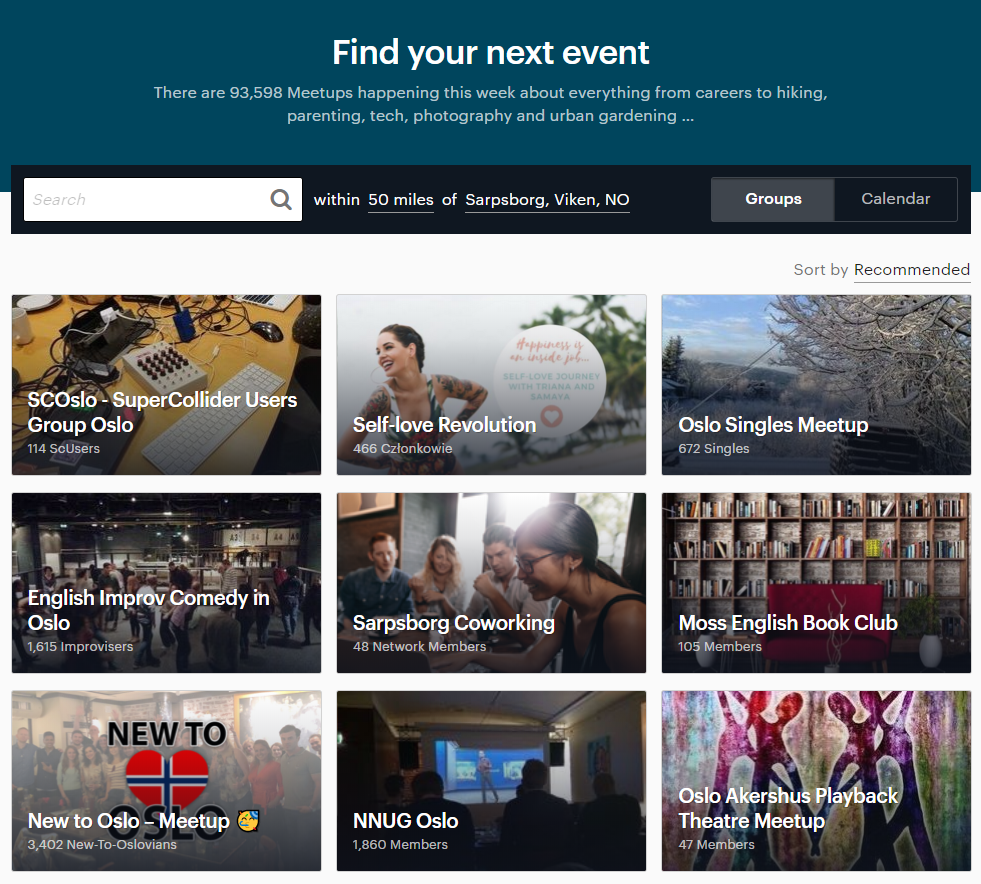
\includegraphics[width=0.48\textwidth]{Illustrasjoner/andre_platformer/meetup_forside.png}
  \end{center}
  \caption{Forsidevisning på Meetup.com etter innlogging.}
\end{wrapfigure}
%END FIGURE%

Etter tvungen brukerregistrering blir man presentert en forside med en rekke kort som representerer relevante aktiviteter for bruker i geografisk område. 
Ved klikk på et av arrangementene møtes man med en informasjonsside som informerer om lokasjon, antall medlemmer, organisator, kommende datoer m.m.

I navigasjonen har bruker tilgang på en utforsk-knapp som går til en søkeside, meldinger fra andre brukere og notifikasjoner om relaterte hendelser.

Prosjektgruppen opplever Meetup.com som en nokså ryddig side, dog med minimal aktivitet i Norge. Det er ingen savn etter ytterligere informasjon fra de ulike arrangementene, og det bør bli vurdert lignende implementasjon ved organisasjonssidene som skal utformes på Aktiv Student.

\paragraph{NyBy} Et verktøy for kommuner og organisasjoner ment for å løse viktige velferdsoppgaver i samarbeid med ansatte og innbyggere. Kommuner legger ut en henvendelse via meldinger på en app, som medlemmer av frivillige organisasjoner i nærheten kan velge å svare på. Målet er mer direkte kommunikasjon mellom behov og støtte, som igjen vil føre til spart tid og kommunale ressurser\footnote{https://nyby.no/hva-er-nyby}.

\begin{figure}[H]
    \centering
    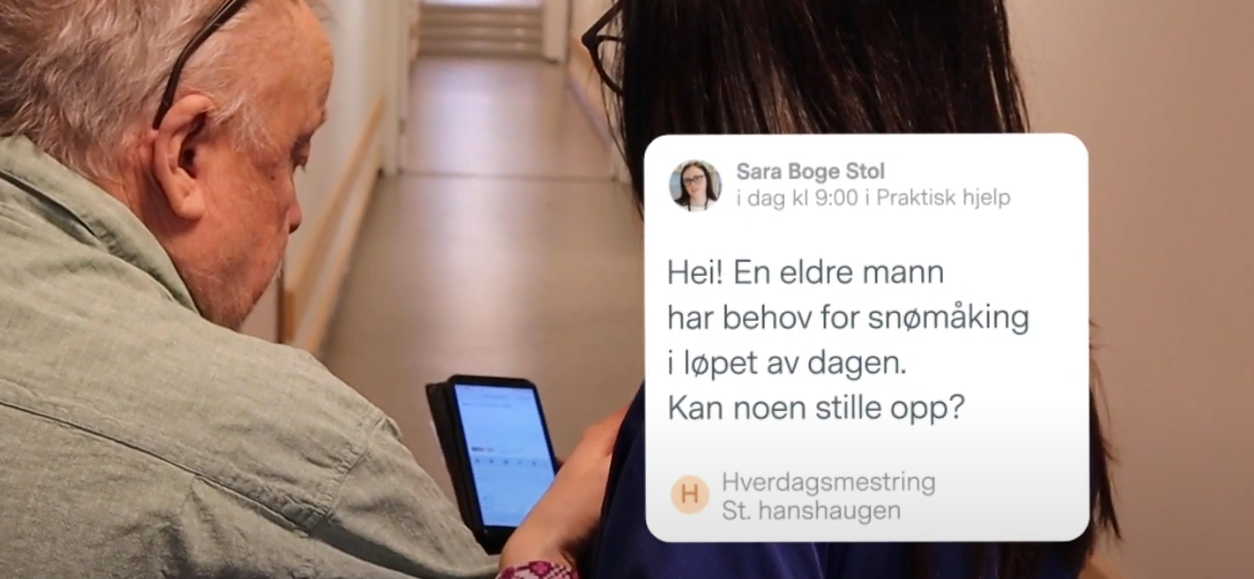
\includegraphics[width=\textwidth]{Illustrasjoner/andre_platformer/nyby_henvendelse.png}
    \caption{Skjermdump fra informasjonsvideo fra nyby.no}
    \label{fig:nyby1}
\end{figure}

%BEGIN FIGURE%
\begin{wrapfigure}{r}{0.5\textwidth}
  \begin{center}
    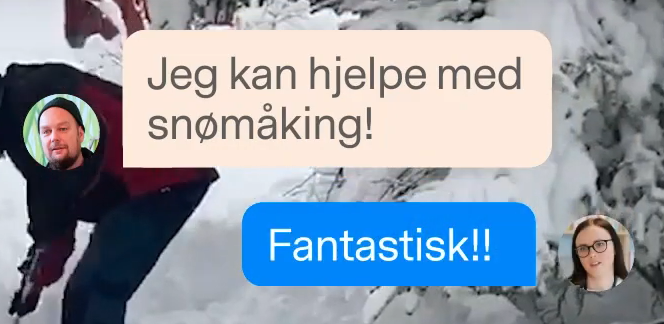
\includegraphics[width=0.48\textwidth]{Illustrasjoner/andre_platformer/nyby_svar.png}
  \end{center}
  \caption{Skjermdump informasjonsvideo fra nyby.no}
  \label{fig:nyby2}
\end{wrapfigure}
%END FIGURE%
Via en app kan de som har behov for hjelp melde seg inn i lokale grupper og spørre om bistand til å gjøre mindre ærender. I samme appen kan de som har mulighet til å hjelpe respondere direkte.

Prosjektgruppen er imponert over effektiviteten over denne type kommunikasjon ved behov for hjelp. Mange mennesker kan få hjelp til ting som for noen er enkle, men for andre særskilt krevende. Dette ved å kutte ut flere ledd innenfor kommunale sektorer, hvor ressursene heller kan prioriteres annerledes. Covid-19 pandemien og dens medfølgende karantenetiltak setter desto større fokus på denne type bidrag til samfunnet.

\paragraph{Nextdoor.com} En tjeneste som setter søkelys på forholdet mellom naboer\footnote{https://global.nextdoor.com/}. Ved registrering kreves verifisering av bostedsadresse, noe som sørger for at brukere kun kan forholde seg til de som bor nær hverandre. Norge er per dags dato ikke et av landene som støttes av Nextdoor, men nettsiden opplyser om et ønske å spre seg til alle land.

Gruppen ser et sterkt fokus på geografisk lokasjon. Selv over nettet så kan miljøet rundt brukere oppfattes veldig personlig, da tjenesten komprimeres kun til de respektive nabolagene.

\paragraph{Frivilligsentral.no} En søkeportal med oversikt over frivillighetsorganisasjoner i Norge. De sørger for inviterende ordbruk, samt en informasjonsrik forside. De har tatt grep for å implementere hvordan Covid-19 forårsaker endringer i deres daglige drift, noe som får de til fremstå som profesjonelle og aktive.

\begin{figure}[H]
\centering
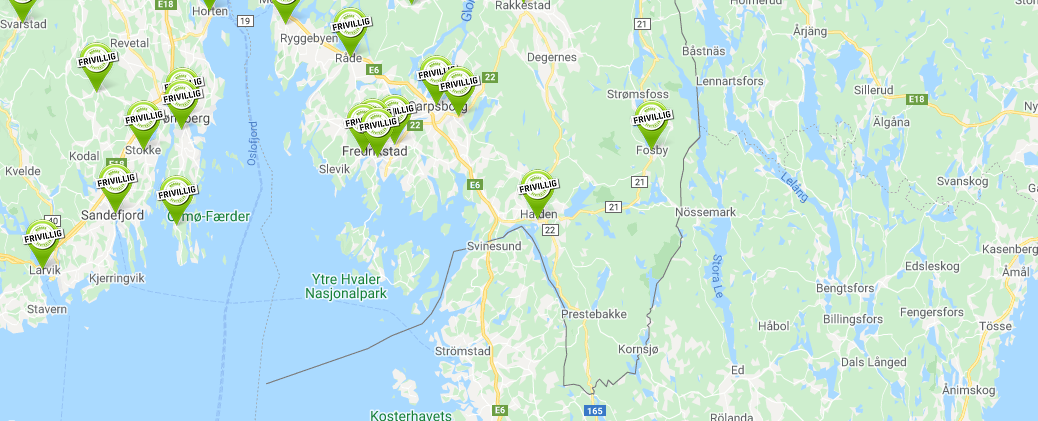
\includegraphics[width=1\textwidth]{Illustrasjoner/frivillig_kart.png}
\caption{Oversikt over lokale organisasjoner hentet fra frivilligsentral.no}
\end{figure}

Besøkende presenteres store mengder statistikk som kan føles overveldende. Tjenesten viser frem statistikk både som tall på forside og under egen lenke, men det kan være gjort for å stadfeste stolthet om hvor mange plasser de holder til. De har et stort og illustrativt norgeskart på forsiden som besøkende kan bruke til å navigere seg til aktuelle organisasjoner for dem.

\paragraph{Oppsummering}
Noe de fleste evaluerte nettsider har til felles, er at de krever registrering og innlogging. Det foreligger som en naturlig funksjon, da de fleste gjøremål trenger identifisering av bruker. Aktiv Student sitt utgangspunkt, frivillighetsregisteret på brreg.no, krever på sin side ingen innlogging. Ved å sammenligne den type innhold med andre generelle oversikter som finnes (finn.no, ut.no, gulesider.no etc), så krever fåtallet av de innlogging. Det forblir da et mål fra prosjektgruppens sin side om å prøve å utelate innlogging, ihvertfall forenkle prosessen betraktelig. Prosjektgruppen diskuterte de forskjellige tjenestene på grunnlag av interessante funksjoner, men også på basis av Jakob Nielsens 10 prinsipper for design av brukergrensesnitt\footnote{https://www.nngroup.com/articles/ten-usability-heuristics/}.


\subsection{Relaterte studier og publikasjoner}
De fleste aspektene med oppdraget er forsket på og skrevet om i studier og publikasjoner. Utvikling av søkemotorer og digitale oppslagsverk er gjort før og det finnes nok av dokumentasjon på dette. Prosjektgruppen valgte derfor å trekke frem de mest sentrale aspektene som, når satt sammen, skiller løsningen beskrevet i oppdraget fra andre tjenester og gir den mulighet til å dekke et behov i markedet. Aspektene som trekkes frem er {\em gjøre det enklere å delta}, {\em oppfordre til deltakelse sammen med andre}, {\em interaksjon med andre brukere} og {\em foreslå aktiviteter for brukerne}. Disse ble undersøkt nærmere ved hjelp av relaterte studier og publikasjoner.

\tittel{Gjøre det enklere å delta}
Målet med oppdraget er å utforme en løsning som gjør det enklere for studenter å finne organisasjoner, lag og foreninger. For å få mer ut av tjenesten vil det også være hensiktsmessig å legge opp til at det skal være enkelt for studentene å ta steget til å faktisk delta på aktiviteter.

Forskningsartikkelen {\em To Go or not to Go!: What Influences Newcomers of Hybrid Communities to Participate Offline} \cite{NEWCOMERS:4:CT17} tar utgangspunkt i tjenesten Meetup.com, beskrevet i delkapittel~\ref{section:relaterte-tjenester}, og undersøker hvilke faktorer som kan spille inn for at brukere skal ta steget fra å passivt benytte tjenesten til å møte opp på en aktivitet for første gang. Funn fra artikkelen peker mot flere faktorer som kan øke sjansen for deltakelse, blant annet {\em utfyllende beskrivelse av arrangementet og instruksjoner for deltakelse
}, {\em at mange andre skulle delta}, {\em inkluderende og velkommende ordbruk i beskrivelsen} og {\em kort sosial distanse mellom bruker og arrangør, slik at det ikke ble truende å ta kontakt}. Disse faktorene ser prosjektgruppen på som relevante for prosjektet og de tas med videre som retningslinjer i utformingen av løsningen.

\tittel{Oppfordre til deltakelse sammen med andre}
Prosjektets sosiale ramme er viktig å ha med seg for å kunne utforme en løsning som gjør det enkelt for studenter å delta i organiserte aktiviteter. Derfor valgte prosjektgruppen å trekke fram aspektet som handlet om det menneskelige aspektet ved organiserte aktiviteter og hvordan digitale løsninger kunne oppfordre brukere til å delta sammen med andre.

Det blir skrevet om digitale tjenester som oppfordrer brukere til å delta på gruppeaktiviteter i {\em Group-Activity Organizing Through an Awareness-of-Others Interface} \cite{AWARENESS:3:CSCW18}. Artikkelen presenterer et brukergrensesnitt som gjør brukere oppmerksom på hverandre gjennom (kalt {\em Awareness-of-Others-Interface} i artikkelen). Gjennom å utvikle en app med utgangspunkt i dette brukergrensesnittet som lar brukere søke opp og organisere gruppeaktiviteter og andre brukere delta på disse, ønsker forskerne å finne ut om dette kan fungere som et verktøy for kollektiv deltakelse. For å bidra til å gjøre brukerne klar over andre brukere i nærheten implementeres det blant annet et komponent i brukergrensesnittet som de kaller {\em Interested People}, som viser brukeren andre brukere i området som har vist interesse for samme aktivitet. Funn i artikkelen viser at synliggjøring av andre interesserte brukere gjennom {\em Interested People}-komponentet økte betydelig sannsynligheten for at brukere valgte å initiere organiseringen av en aktivitet. Derimot var det ingenting som pekte mot at brukene ble mer motiverte til å bidra til å faktisk gjennomføre organiseringen. Det viktigste punktet å ta med seg videre i utformingen herifra er hvordan synliggjøring av andre brukere i en tjeneste kan øke muligheten til at bruker velger å delta sammen med andre.

\tittel{Interaksjon med andre brukere}
For å bygge videre på de sosiale rammene ønsket prosjektgruppen å undersøke hvordan interaksjon mellom brukere kan oppfordres. Å oppfordre brukere til å snakke med ukjente eller personer de ikke kjenner så godt kan bli utfordrende. Aspektet som handler om å gi brukere en grunn til å interagere og samtidig senke terskelen for dette trekkes derfor frem.

Forskningsartikkelen {\em Outlining the design space of playful interactions between nearby strangers}  beskriver en designprosess med workshops for å utvikle idéer til hvordan teknologi kan oppfordre fremmede mennesker som befinner seg i nærheten av hverandre kan interagere på forskjellige måter. I artikkelen beskrives forskjellige nivåer av interaksjon mellom brukere blant idéene fra automatisk utveksling av informasjon mellom enheter til at brukere samarbeider om en oppgave. Forfatterne skriver dette om å senke terskelen for interaksjon gjennom teknologi \say{Technology can announce and enforce rules that lower the threshold to interact by defining what is expected from people and how they are supposed to behave during encounters.} \cite{NEARBY:5:AM16}. 

Videre er forskningsartikkelen {\em Playfulness and progression in technology-enhanced social experiences between nearby strangers}  en videreføring av designprosessen i {\em Outlining the design space of playful interactions between nearby strangers}, der forskerne utvikler en app som heter Next2You etter prinsippene {\em lekenhet} og {\em progresjon}. Appen lar brukerne automatisk utveksle valgfri informasjon med andre brukere som kommer innen mobiltelefonens Bluetooth-radius. Appen blir testet på brukere i et studie for å finne ut om de to prinsippene {\em lekenhet} og {\em progresjon} kan bidra til å oppfordre til interaksjon mellom brukere. Resultatene fra forskningen peker i retning mot at bruk av appen oppfordret til interaksjon mellom brukere som ikke ville funnet sted uten. I tillegg konkluderer artikkelen med designhensyn for videre arbeid innenfor dette fagområdet: {\em styrke muligheten for møter mellom brukere}, {\em oppfordre til brukergenerert innhold med høy kvalitet}, {\em oppfordre til større engasjement mellom brukere og tjenesten}.\cite{PLAYFUL:6:NORDICHI18}.

Prinsippene lekenhet og progresjon er prinsipper som også går an å benytte i utformingen av prosjektgruppens løsning. I tillegg vil det være viktig å tenke på hvilke hensyn som kan tas i designet for å senke terskelen for interaksjon med andre brukere. 

\tittel{Foreslå aktiviteter for brukere}
Det er ønskelig å utforme en løsning som gjør det både enkelt og spennende for studenter å finne aktivitetstilbud, samt å gi brukerne flere valgmuligheter som de kanskje ikke ville funnet på egen hånd. Derfor undersøkes metoder og arbeid som handler om å foreslå aktiviteter til brukerne basert på informasjon om dem.

Anbefaling av aktiviteter er skrevet om i forskningsartikkelen {\em A Novel Method for Event Recommendation in Meetup}. Her beskrives utviklingen av en formel for å effektivt kunne anbefale brukeren arrangementer til en bruker av Meetup.com. Formelen tar utgangspunkt i interessene til brukere som deltar på arrangementer sammen for å kunne presentere forslag til andre brukere. Formelen ble deretter testet i Meetup.com og hadde en høy suksessrate i å foreslå arrangementer til brukere som de valgte å delta på. \cite{MEETUP:7:ASONAM17}. Aspektet med å foreslå aktiviteter til brukere gjennom andre brukere er en idé prosjektgruppen mener kan være relevant å se videre på i utformingen av løsningen.

{\em Users psychological profiles for leisure activity recommendation: user study} beskriver et brukerstudie som bruker brukernes selvrapporterte personlighetstrekk og informasjon om hva som er viktig for fritiden deres for å kartlegge mønster som senere kan brukes til å anbefale aktiviteter for andre brukere på grunnlag av personlighetstrekk. Studiet kom fram til en stor mengde korrelasjoner mellom personlighetstrekk og hvilke typer aktiviteter brukerne var interessert i. \cite{PROFILES:10:CITREC17}. Selv om en omfattende personlighetstest ikke er gjennomførbart eller hensiktsmessig er denne måten å korrelere mellom personlighet, ønsker og fritidsaktiviteter på interessant for prosjektgruppen. 

\tittel{Oppsummering}
Gjennom å se videre på disse aspektene og sette dem sammen har prosjektgruppen et utgangspunkt for arbeidet med utformingen av et konsept og medfølgende prototype for Aktiv Student. Med et overordnet mål om å bidra til å utforme en løsning for å finne lokale aktivitetstilbud som både er brukervennlig, fornøyelig å bruke og sosial vil prosjektet kunne bidra til å fylle et behov i markedet og kunne bli mer enn kun et digitalt oppslagsverk, men en {\em bevegelse} for aktivisering av studenter.

\section{Rapportstruktur}
\paragraph{Kapittel 2} Inneholder en beskrivelse av arbeidsprosessen med billedlig og skriftlig dokumentasjon, brukerundersøkelser, utvikling av skisser, brukertesting, evalueringer og forbedringer som er gjort.

\paragraph{Kapittel 3}
Inneholder en beskrivelse av det det ferdige resultatet som gruppen produserte og en evaluering av dette fra studenter, organisasjoner, personer innenfor fagfeltet og oppdragsgiver.

\paragraph{Kapittel 4}
Diskuterer resultatet i henhold til oppnåelsen av krav og spesifikasjoner satt på forhånd. Her vil det foreligge en vurdering av prosjektet og arbeidet fra prosjektgruppen og anbefalinger samt designprinsipper for videre arbeid. Gruppen vil også diskutere erfaringer gjort underveis i arbeidet. Avslutningsvis legges det frem en konklusjon og oppsummering.

